\chapter*{Лабораторная работа 3. Шифрование сообщений с помощью средств GNU Privacy Guard}
\addcontentsline{toc}{chapter}{Лабораторная работа 3. Шифрование сообщений с помощью средств GNU Privacy Guard}

\textbf{Цель работы:} Знакомство с возможностями утилиты GNU Privacy Guard.

\section*{1. Установка}
\addcontentsline{toc}{section}{1. Установка}
Установка утилиты не потребовалась, т.к. она уже установлена на компьютере.
\begin{Verbatim}[frame=single]
    smart@thinkpad$ pacman -Qi gnupg
    Name            : gnupg
    Version         : 2.2.40-1
    Description     : Complete and free implementation of the OpenPGP standard
    Architecture    : x86_64
    URL             : https://www.gnupg.org/
    Licenses        : BSD  custom  custom:CC0  GPL2  GPL3  LGPL3  LGPL2.1  MIT
    Groups          : None
    Provides        : None
    Depends On      : bzip2  libbz2.so=1.0-64  glibc  gnutls  libgcrypt
                      libgpg-error  libksba  libassuan  libassuan.so=0-64  npth
                      libnpth.so=0-64  pinentry  readline  libreadline.so=8-64
                      sqlite  zlib
    Optional Deps   : libldap: gpg2keys_ldap [installed]
                      libusb-compat: scdaemon
                      pcsclite: scdaemon [installed]
    Required By     : gpgme  pacman  visual-studio-code-bin
    Optional For    : None
    Conflicts With  : None
    Replaces        : None
    Installed Size  : 8.55 MiB
    Packager        : David Runge <dvzrv@archlinux.org>
    Build Date      : Fri 14 Oct 2022 02:01:35 PM MSK
    Install Date    : Mon 19 Dec 2022 11:46:09 PM MSK
    Install Reason  : Installed as a dependency for another package
    Install Script  : Yes
    Validated By    : Signature
\end{Verbatim}

Информация о текущей версии \texttt{GnuPG} и поддерживаемых криптоалгоритмах
\begin{Verbatim}[frame=single]
    smart@thinkpad$ gpg2 --version
    gpg (GnuPG) 2.2.40
    libgcrypt 1.10.1-unknown
    Copyright (C) 2022 g10 Code GmbH
    License GNU GPL-3.0-or-later <https://gnu.org/licenses/gpl.html>
    This is free software: you are free to change and redistribute it.
    There is NO WARRANTY, to the extent permitted by law.

    Home: /home/smart/.gnupg
    Supported algorithms:
    Pubkey: RSA, ELG, DSA, ECDH, ECDSA, EDDSA
    Cipher: IDEA, 3DES, CAST5, BLOWFISH, AES, AES192, AES256, TWOFISH,
            CAMELLIA128, CAMELLIA192, CAMELLIA256
    Hash: SHA1, RIPEMD160, SHA256, SHA384, SHA512, SHA224
    Compression: Uncompressed, ZIP, ZLIB, BZIP2
\end{Verbatim}

\section*{2. Генерация ключей}
\addcontentsline{toc}{section}{2. Генерация ключей}
Произведём генерацию ключей.

Для диалога генерации ключа я использую флаг \texttt{--full-generate-key}, т.к. стандартный \texttt{--gen-key} скрывает некоторые вопросы диалога используя значения по умолчанию (в частности, используется ключ длинной 3072).
\begin{Verbatim}[frame=single]
    smart@thinkpad$ gpg2 --full-generate-key
    gpg (GnuPG) 2.2.40; Copyright (C) 2022 g10 Code GmbH
    This is free software: you are free to change and redistribute it.
    There is NO WARRANTY, to the extent permitted by law.
    
    Please select what kind of key you want:
       (1) RSA and RSA (default)
       (2) DSA and Elgamal
       (3) DSA (sign only)
       (4) RSA (sign only)
      (14) Existing key from card
    Your selection? 1
    RSA keys may be between 1024 and 4096 bits long.
    What keysize do you want? (3072) 4096
    Requested keysize is 4096 bits
    Please specify how long the key should be valid.
             0 = key does not expire
          <n>  = key expires in n days
          <n>w = key expires in n weeks
          <n>m = key expires in n months
          <n>y = key expires in n years
    Key is valid for? (0) 3w
    Key expires at Sat 04 Mar 2023 05:10:43 PM MSK
    Is this correct? (y/N) y
    
    GnuPG needs to construct a user ID to identify your key.
    
    Real name: Semen Martynov
    Email address: martynov.sa@edu.spbstu.ru
    Comment: Test digital sirnature
    You selected this USER-ID:
        "Semen Martynov (Test digital sirnature) <martynov.sa@edu.spbstu.ru>"
    
    Change (N)ame, (C)omment, (E)mail or (O)kay/(Q)uit? O
    We need to generate a lot of random bytes. It is a good idea to perform
    some other action (type on the keyboard, move the mouse, utilize the
    disks) during the prime generation; this gives the random number
    generator a better chance to gain enough entropy.
    We need to generate a lot of random bytes. It is a good idea to perform
    some other action (type on the keyboard, move the mouse, utilize the
    disks) during the prime generation; this gives the random number
    generator a better chance to gain enough entropy.
    gpg: /home/smart/.gnupg/trustdb.gpg: trustdb created
    gpg: directory '/home/smart/.gnupg/openpgp-revocs.d' created
    gpg: revocation certificate stored as '/home/smart/.gnupg/openpgp-revocs.d/9DAF94FCD9CA38BFD298BD0CA0B01E0BAB2AF7C6.rev'
    public and secret key created and signed.
    
    pub   rsa4096 2023-02-11 [SC] [expires: 2023-03-04]
          9DAF94FCD9CA38BFD298BD0CA0B01E0BAB2AF7C6
    uid                      Semen Martynov (Test digital sirnature) <martynov.sa@edu.spbstu.ru>
    sub   rsa4096 2023-02-11 [E] [expires: 2023-03-04]
\end{Verbatim}

В режиме диалога, были выбраны следующие опции
\begin{itemize}
    \item Использование ключа с двумя типа шифрования (RSA и RSA)
    \item Длинна ключа в 4096 бит (с 2015-го года NIST рекомендует использовать ключи длинной в 2018 бит, но уже сейчас многие компании перешли на 4096)
    \item 3 недели в качестве срока жизни ключа (как долго он будет валиден для использования)
    \item Имя и e-main предоставленный университетом.
\end{itemize}

Дальше выполнение диалога прервалось для ввода ключевой фразы, защищающей ключи от несанкционированного использования.
\begin{center}
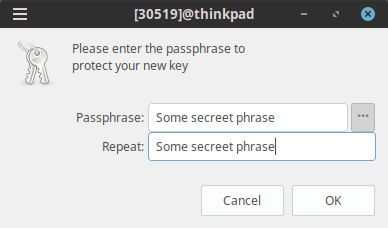
\includegraphics[scale=0.8]{res/3.pass1.png}
\end{center}

Был выбран слабый пароль для шифрования, о чём система меня предупредила. Продолжим с небезопасным паролем.
\begin{center}
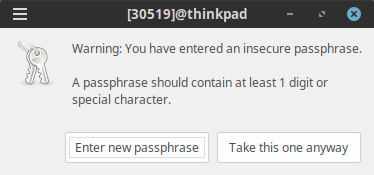
\includegraphics[scale=0.8]{res/3.pass2.png}
\end{center}

Текущий список ключей с keygrip (идемпотентный протокол хеширования для связи ключей)
\begin{Verbatim}[frame=single]
    smart@thinkpad$ gpg --list-keys --with-keygrip
    /home/smart/.gnupg/pubring.kbx
    ------------------------------
    pub   rsa4096 2023-02-11 [SC] [expires: 2023-03-04]
          9DAF94FCD9CA38BFD298BD0CA0B01E0BAB2AF7C6
          Keygrip = EC3AFAA6FD0AE71FB449D7D42849E173CF6CAAF4
    uid           [ultimate] Semen Martynov (Test digital sirnature) <martynov.sa@edu.spbstu.ru>
    sub   rsa4096 2023-02-11 [E] [expires: 2023-03-04]
          Keygrip = 16E5EFCBA47102BBA3A7C17D467D430C13D3D43E
\end{Verbatim}

\begin{itemize}
    \item \texttt{pub} -- публичный ключ (keygrip \texttt{EC3AFAA6FD0AE71FB449D7D42849E173CF6CAAF4});
    \item \texttt{uid} -- идентификатор (User-ID);
    \item \texttt{sub} -- публичный подключ (keygrip \texttt{16E5EFCBA47102BBA3A7C17D467D430C13D3D43E});
\end{itemize}

Список приватных ключей
\begin{Verbatim}[frame=single]
    smart@thinkpad$ gpg2 --list-secret-keys --with-keygrip
    /home/smart/.gnupg/pubring.kbx
    ------------------------------
    sec   rsa4096 2023-02-11 [SC] [expires: 2023-03-04]
        9DAF94FCD9CA38BFD298BD0CA0B01E0BAB2AF7C6
        Keygrip = EC3AFAA6FD0AE71FB449D7D42849E173CF6CAAF4
    uid           [ultimate] Semen Martynov (Test digital sirnature) <martynov.sa@edu.spbstu.ru>
    ssb   rsa4096 2023-02-11 [E] [expires: 2023-03-04]
        Keygrip = 16E5EFCBA47102BBA3A7C17D467D430C13D3D43E
\end{Verbatim}

\begin{itemize}
    \item \texttt{sec} -- секретный ключ (keygrip \texttt{EC3AFAA6FD0AE71FB449D7D42849E173CF6CAAF4});
    \item \texttt{uid} -- идентификатор (User-ID);
    \item \texttt{ssb} -- секретный подключ (keygrip \texttt{16E5EFCBA47102BBA3A7C17D467D430C13D3D43E});
\end{itemize}

Список подписей
\begin{Verbatim}[frame=single]
    smart@thinkpad$ gpg2 --list-signatures --with-keygrip
    /home/smart/.gnupg/pubring.kbx
    ------------------------------
    pub   rsa4096 2023-02-11 [SC] [expires: 2023-03-04]
        9DAF94FCD9CA38BFD298BD0CA0B01E0BAB2AF7C6
        Keygrip = EC3AFAA6FD0AE71FB449D7D42849E173CF6CAAF4
    uid           [ultimate] Semen Martynov (Test digital sirnature) <martynov.sa@edu.spbstu.ru>
    sig 3        A0B01E0BAB2AF7C6 2023-02-11  Semen Martynov (Test digital sirnature) <martynov.sa@edu.spbstu.ru>
    sub   rsa4096 2023-02-11 [E] [expires: 2023-03-04]
        Keygrip = 16E5EFCBA47102BBA3A7C17D467D430C13D3D43E
    sig          A0B01E0BAB2AF7C6 2023-02-11  Semen Martynov (Test digital sirnature) <martynov.sa@edu.spbstu.ru>
\end{Verbatim}

Отпечаток (fingerprint) подписи
\begin{Verbatim}[frame=single]
    smart@thinkpad$ gpg2 --fingerprint martynov.sa@edu.spbstu.ru
    pub   rsa4096 2023-02-11 [SC] [expires: 2023-03-04]
          9DAF 94FC D9CA 38BF D298  BD0C A0B0 1E0B AB2A F7C6
    uid           [ultimate] Semen Martynov (Test digital sirnature) <martynov.sa@edu.spbstu.ru>
    sub   rsa4096 2023-02-11 [E] [expires: 2023-03-04]
\end{Verbatim}

Исследуем содержимое директории \texttt{.gnupg}
\begin{Verbatim}[frame=single]
smart@thinkpad$ tree .gnupg/
.gnupg/
    openpgp-revocs.d
        9DAF94FCD9CA38BFD298BD0CA0B01E0BAB2AF7C6.rev
    private-keys-v1.d
        16E5EFCBA47102BBA3A7C17D467D430C13D3D43E.key
        EC3AFAA6FD0AE71FB449D7D42849E173CF6CAAF4.key
    pubring.kbx
    pubring.kbx~
    trustdb.gpg
\end{Verbatim}

В директории можно увидеть
\begin{itemize}
    \item \texttt{openpgp-revocs.d/9DAF94FCD9CA38BFD298BD0CA0B01E0BAB2AF7C6.rev} --  предварительно созданный сертификат отзыва. Имя файла соответствует отпечатку ключа. Всякий, у кого есть доступ к этому файлу, может отозвать соответствующий ключ.
    \item \texttt{private-keys-v1.d/EC3AFAA6FD0AE71FB449D7D42849E173CF6CAAF4.key} -- приватный ключ.
    \item \texttt{private-keys-v1.d/16E5EFCBA47102BBA3A7C17D467D430C13D3D43E.key} -- приватный подключ.
    \item \texttt{pubring.kbx} -- Таблица открытых ключей.
    \item \texttt{pubring.kbx~} -- Таблица открытых ключей (резервная копия).
    \item \texttt{trustdb.gpg} -- База данных доверия (Алиса подписала публичный ключ Боба, а Боб подписал публичный ключ Чарли; если Алиса получит публичный ключ Чарли, она сможет ему доверять, потому что ключ подписан тем, кому Алиса доверяет, т.е. Бобом).
\end{itemize}

\section*{3. Шифрование и подпись текста}
\addcontentsline{toc}{section}{3. Шифрование и подпись текста}
Для демонстрации возможностей утилиты, сгенерируем простой \texttt{Lorem Ipsum}.
\lstinputlisting[caption={Lorem Ipsum}, numbers=none]
{../Tasks/3_4_GnuPG_tool_utilisation/source_files/LoremIpsum.txt}

Теперь зашифруем файл с тестовым выводом
\begin{Verbatim}[frame=single]
    smart@thinkpad$ gpg2 \
     --armor \
     --recipient 9DAF94FCD9CA38BFD298BD0CA0B01E0BAB2AF7C6 \
     --encrypt LoremIpsum.txt
\end{Verbatim}

\lstinputlisting[caption={зашифрованный Lorem Ipsum}, numbers=none]
{../Tasks/3_4_GnuPG_tool_utilisation/source_files/LoremIpsum.txt.asc.nosign}

Далее расшифруем файл (операция потребует ввода приватной фразы!)
\begin{Verbatim}[frame=single]
    smart@thinkpad$ gpg2 \
     --recipient 9DAF94FCD9CA38BFD298BD0CA0B01E0BAB2AF7C6 \
     --decrypt LoremIpsum.txt.asc > LoremIpsum.decrypted.txt
\end{Verbatim}

Убедимся, что расшифрованный файл соответствует исходному.
\begin{Verbatim}[frame=single]
    smart@thinkpad$ shasum -a 1 LoremIpsum.txt LoremIpsum.decrypted.txt 
    014bbacd9d092d1f2272a3419125dbb2de0f3a6b  LoremIpsum.txt
    014bbacd9d092d1f2272a3419125dbb2de0f3a6b  LoremIpsum.decrypted.txt
\end{Verbatim}

\begin{Verbatim}[frame=single]
    smart@thinkpad$ gpg2 \
     --recipient 9DAF94FCD9CA38BFD298BD0CA0B01E0BAB2AF7C6 \
     --clearsign LoremIpsum.txt
\end{Verbatim}

\lstinputlisting[caption={Lorem Ipsum с цифровой подписью}, numbers=none]
{../Tasks/3_4_GnuPG_tool_utilisation/source_files/LoremIpsum.txt.asc}

Проверка цифровой подписи
\begin{Verbatim}[frame=single]
    smart@thinkpad$ gpg2 --verify LoremIpsum.txt.asc
    gpg: Signature made Sat 11 Feb 2023 07:57:52 PM MSK
    gpg:                using RSA key 9DAF94FCD9CA38BFD298BD0CA0B01E0BAB2AF7C6
    gpg: Good signature from "Semen Martynov (Test digital sirnature) <martynov.sa@edu.spbstu.ru>" [ultimate]
\end{Verbatim}

\section*{4. Прочие возможности использования GPG}
\addcontentsline{toc}{section}{4. Прочие возможности использования GPG}
Популярным способом использования GPG является цифровая подпись коммитов в git. Для этого в \texttt{.gitconfig} нужно добавить следующие параметры
\begin{Verbatim}[frame=single]
[commit]
        gpgsign = true
[user]
        signingkey = <KeyID>
[gpg]
        program = /bin/gpg
\end{Verbatim}

\section*{Выводы}
\addcontentsline{toc}{section}{Выводы}

В данной работе мы провели знакомство с возможностями утилиты GNU Privacy Guard. Разобрались с процессом генерации ключей и их хранением. Выполнили шифрование и сделали цифровую (присоединенную) подпись документа.

В практическом плане, использование GNU Privacy Guard позволяет подписывать коммитов в git для однозначного установления авторства.
